%
% mtexamples2.tex
%
% (c) 2023 Prof Dr Andreas Müller
%
\begin{figure}
\centering
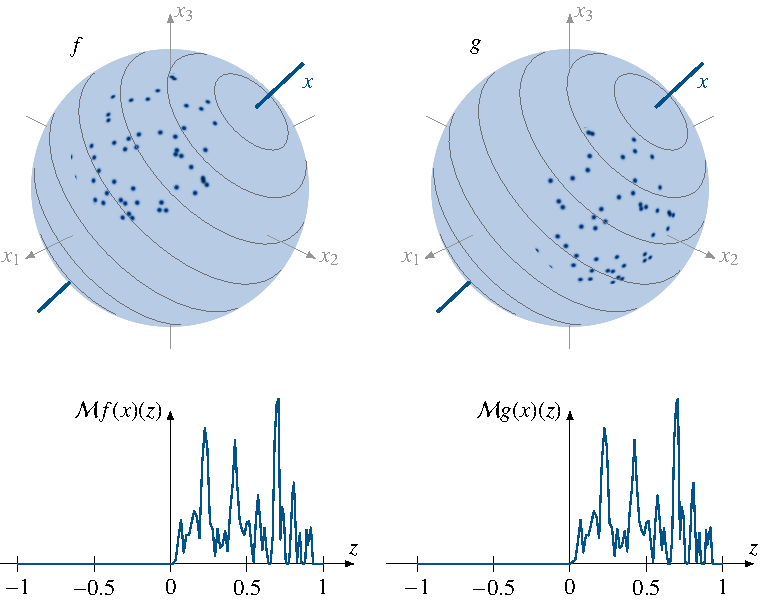
\includegraphics{chapters/070-nichtkomm/images/MTransformExamples2.pdf}
\caption{Méndez-Transformation der zwei Funktionen $f$ und $g$ auf
der Kugeloberfläche.
Die Achse mit Richtungsvektor $x$ gehört zu derjenigen Drehung,
die $f$ in $g$ überführt.
Die Méndez-Transformationen $\mathcal{M}f(x)$
und $\mathcal{M}g(x)$ sind gleich.
\label{buch:nichtkomm:fig:mtex2}}
\end{figure}
